\documentclass[journal]{IEEEtran}
\usepackage{amsmath,amssymb,amsthm}
\usepackage{bm}
\usepackage{graphicx}
\usepackage{booktabs}
\usepackage{array}
\usepackage{cite}
\usepackage[colorlinks=false,pdfborder={0 0 0}]{hyperref}

\newtheorem{theorem}{Theorem}
\newtheorem{lemma}{Lemma}
\newtheorem{proposition}{Proposition}
\newtheorem{remark}{Remark}

\newcommand{\zv}{\mathbf{z}}
\newcommand{\uv}{\mathbf{u}}
\newcommand{\bv}{\mathbf{b}}
\newcommand{\nv}{\mathbf{n}}
\newcommand{\tv}{\mathbf{t}}
\newcommand{\vv}{\mathbf{v}}
\newcommand{\phiv}{\bm{\varphi}}
\newcommand{\Jc}{\mathcal{J}}
\newcommand{\Lc}{\mathcal{L}}
\newcommand{\atan}{\operatorname{atan2}}
\newcommand{\T}{\mathsf{T}}

\begin{document}

\title{An Exact Affine Framework for Arbitrary-Point Bias Control of
Mach--Zehnder and Dual-Parallel Mach--Zehnder Modulators}

\author{First~A.~Author,~Second~B.~Author%
\thanks{Manuscript draft. Author names, affiliations, and funding
information to be completed. The authors are with the State Key Laboratory
of Integrated Service Networks, Xidian University, Xi'an 710071, China.}}

\markboth{Preprint --- Affine Framework for MZM/DPMZM Bias Control}%
{Author \MakeLowercase{\textit{et al.}}: Exact Affine Framework for Arbitrary-Point Bias Control}

\maketitle

\begin{abstract}
Pilot-tone bias controllers for Mach--Zehnder modulators (MZMs)
traditionally lock only a handful of special operating points
(quadrature, null, peak), because every scalar harmonic error signal
necessarily exhibits dead zones and branch ambiguities over a full bias
period. This paper establishes an \emph{exact} structural theorem: for an
arbitrary periodic dither waveform and an arbitrary linear receive chain,
the vector of harmonically demodulated observables is an affine image of
the unit circle $\mathbb{S}^1$ parameterized by the bias phase. All
linear impairments---gain imbalance, reference-phase errors, dither
waveform distortion, coherent crosstalk, finite extinction ratio---only
relocate the affine parameters $(A,\bv)$ and never alter the model form.
Arbitrary-point bias control thereby reduces to ellipse identification
(a Heydemann-type correction transplanted to the bias domain, with a
regression-based gauge fixing that avoids the ill-conditioned flat
minimum of the dc fiducial) followed by direct $\atan$ phase
demodulation, yielding a control loop whose gain is uniform over the
entire period. The static errors of all conventional schemes are derived
in closed form as ratios of affine entries. The framework is then
extended to the dual-parallel MZM (DPMZM): the state manifold becomes the
3-torus $\mathbb{T}^3$, and exact affinity survives through a 12-dimensional
trigonometric feature map containing half-angle terms. The half-angle
structure implies a $4\pi$ calibration period, a Klein four-group
configuration equivalence, and---most consequentially---an observability
theorem proving that the singular set of the six harmonic channels is
precisely the Klein orbit of the standard QPSK operating point, so that
intermodulation-tone detection of the parent bias is a rank-condition
necessity rather than an engineering heuristic. Calibration generalizes
to linear regression over a single quasi-periodic space-filling sweep,
and demodulation to a warm-started Gauss--Newton iteration costing under
$10^3$ multiply--accumulates per control cycle. Numerical validation
shows machine-precision closure in the noiseless limit, millradian-level
residuals under realistic noise, and one to two orders of magnitude
improvement over conventional multi-loop locking at arbitrary targets,
where conventional loops exhibit static errors of hundreds of mrad or
lose lock entirely.
\end{abstract}

\begin{IEEEkeywords}
Mach--Zehnder modulator, dual-parallel MZM, bias control, pilot tone,
affine identification, ellipse fitting, observability, Gauss--Newton,
microwave photonics.
\end{IEEEkeywords}

\IEEEpeerreviewmaketitle

\section{Introduction}
\IEEEPARstart{L}{ithium}-niobate and InP Mach--Zehnder modulators (MZMs)
suffer slow bias drift caused by temperature, charge accumulation, and
photorefractive effects \cite{salvestrini2011,chen2011}. Closed-loop bias
controllers based on a small low-frequency pilot tone (dither) are the
de-facto standard: the first and second harmonics of the detected
photocurrent provide error signals that vanish at the null/peak and
quadrature points respectively, and decades of refinement have produced
robust special-point locking for on--off keying as well as multi-loop
extensions for IQ and dual-polarization transmitters
\cite{cho2006,sotoodeh2011,kawakami2012}.

A growing class of applications, however, requires the bias to be
parked at an \emph{arbitrary} phase: microwave-photonic phase shifters
and vector modulators, single-sideband weight control, analog photonic
computing, and chirp management all demand continuous setpoints on the
transfer curve. Conventional practice extrapolates the special-point
machinery in one of two ways---matching a harmonic amplitude to a
nominal reference, or forming the ratio of two harmonics---and both
inherit structural defects: vanishing loop gain near specific phases
(dead zones), $\varphi\leftrightarrow\pi-\varphi$ branch ambiguity, and
first-order sensitivity to gain calibration that the original
zero-crossing schemes were immune to. For the dual-parallel MZM (DPMZM),
the difficulty compounds: the three bias loops couple through the parent
interferometer, and the textbook decoupled-loop design is only valid in
a neighborhood of the standard QPSK point.

This paper argues that these are not isolated engineering nuisances but
projections of a single geometric fact, and that recognizing the fact
yields a complete arbitrary-point solution. The contributions are:

\begin{enumerate}
\item \emph{An exact affine theorem (single MZM).} For any periodic
dither waveform and any linear receive chain, the demodulated observable
vector satisfies $\zv = A\uv(\varphi_b)+\bv+\nv$ \emph{exactly}, with
$\uv=(\cos\varphi_b,\sin\varphi_b)^{\T}$. Closed-form expressions of
$A$, $\bv$, $\nv$ in conventional pilot-tone quantities are given,
including the $O(\varepsilon)$ off-diagonal entries generated by dither
second-harmonic distortion (Appendix~\ref{app:eps}).
\item \emph{Conventional schemes as degenerate readouts.} The static
locking errors of quadrature, null/peak, amplitude-matching, and
harmonic-ratio schemes are derived in closed form as ratios of affine
entries, unifying scattered error analyses
(Table~\ref{tab:schemes}).
\item \emph{Self-calibrating arbitrary-point control.} Ellipse
identification with a full-curve dc-regression gauge fixing (shown to
reduce the gauge variance by $\mathcal{O}(1/N)$ relative to the
ill-conditioned argmin fiducial), $\atan$ demodulation, and a control
loop with target-independent gain.
\item \emph{Exact DPMZM generalization.} A 12-dimensional trigonometric
feature map $\Phi:\mathbb{T}^3\to\mathbb{R}^{12}$ with half-angle
structure preserves exact affinity; the $4\pi$ child-axis period and the
Klein four-group configuration equivalence follow.
\item \emph{An observability theorem.} The singular set of the six
harmonic channels is exactly the Klein orbit of the standard QPSK
point---the conventional channel set is blind precisely where everyone
operates---and the intermodulation (IMD) channels
$\omega_1\!\pm\!\omega_2$ used heuristically in the literature
\cite{kawakami2012} are proved to be a rank-condition necessity. A
residual singularity of the nine-channel set at
$\{c_1{=}c_2{=}0,\ \sin\varphi_3{=}0\}$ is identified.
\item \emph{Scalable algorithms.} Calibration by linear regression over
a single quasi-periodic space-filling sweep, and demodulation by
warm-started damped Gauss--Newton, both compatible with Cortex-M class
microcontrollers. All claims are validated numerically to machine
precision in the noiseless limit.
\end{enumerate}

The single-MZM identification step is mathematically a Heydemann
correction \cite{heydemann1981,fitzgibbon1999} transplanted from
displacement interferometry to the bias domain and fused with the
control law; the DPMZM step shows what survives of that picture when
the model surface ceases to be a quadric.

Section~II reviews the signal model and conventional locking;
Sections~III--V develop the single-MZM theory; Sections~VI--VIII develop
the DPMZM extension; Section~IX reports numerical validation;
Section~X discusses limitations and the DP-QPSK case.

\section{Signal Model and Conventional Pilot-Tone Locking}
\label{sec:model}

\subsection{Model and Demodulation Functionals}
Consider a push--pull single-drive MZM with arm power-split ratio $r$,
\begin{equation}
P_{\mathrm{out}}(t)=\tfrac{P_0}{2}\bigl[1+\eta\cos\varphi(t)\bigr],\quad
\eta=\tfrac{2\sqrt r}{1+r}\le 1,
\label{eq:mzm}
\end{equation}
with $\varphi(t)=\varphi_b+\xi(t)$,
$\varphi_b=\pi V_b/V_\pi+\varphi_0$, and nominal dither
$\xi(t)=m\sin\omega t$, $m=\pi V_d/V_\pi$. Constant chirp phase is
absorbed into $\varphi_0$. The photocurrent decomposes as
$i(t)=\rho P_{\mathrm{out}}(t)+i_x(t)+i_n(t)$, where $i_x$ collects
deterministic electrical crosstalk \emph{coherent} with the dither and
$i_n$ is a stochastic noise process. Lock-in demodulation is modeled by
the linear functionals
\begin{equation}
\Lc_1[f]\!\triangleq\!\overline{2f(t)\sin(\omega t{+}\theta_1)},\quad
\Lc_2[f]\!\triangleq\!\overline{2f(t)\cos(2\omega t{+}\theta_2)},
\label{eq:lockin}
\end{equation}
where the overline denotes the low-pass time average and
$\theta_1,\theta_2$ are reference-phase errors (including chain group
delay). With electronic gains $G_1,G_2$ the observables are
$Y\triangleq G_1\Lc_1[i]$ and $X\triangleq G_2\Lc_2[i]$.

The Jacobi--Anger expansion of $\cos(\varphi_b+m\sin\omega t)$ yields
the harmonic structure of Table~\ref{tab:harm}: even harmonics carry
$\cos\varphi_b$ with coefficients $J_{2k}(m)$, odd harmonics carry
$\sin\varphi_b$ with $J_{2k+1}(m)$, and the dc term carries
$1+\eta J_0(m)\cos\varphi_b$. In the ideal limit
($\theta_i{=}0$, sinusoidal $\xi$, $i_x{=}0$),
\begin{equation}
Y=-\eta\kappa_1\sin\varphi_b,\quad X=\eta\kappa_2\cos\varphi_b,\quad
\kappa_n\triangleq G_n\rho P_0 J_n(m),
\label{eq:ideal}
\end{equation}
where $\kappa_1,\kappa_2$ are the familiar harmonic slope
coefficients of the pilot-tone literature.

\begin{table}[!t]
\caption{Harmonic Structure of the Dithered MZM Photocurrent}
\label{tab:harm}
\centering
\begin{tabular}{llll}
\toprule
Freq. & Photocurrent component & $\varphi_b$ dep. & Conventional use\\
\midrule
dc & $\frac{\rho P_0}{2}[1{+}\eta J_0(m)\cos\varphi_b]$ & $\cos\varphi_b$ & power monitor; gauge\\
$\omega$ & $-\eta\rho P_0 J_1(m)\sin\varphi_b$ & $\sin\varphi_b$ & null/peak lock\\
$2\omega$ & $+\eta\rho P_0 J_2(m)\cos\varphi_b$ & $\cos\varphi_b$ & quadrature lock\\
$3\omega$ & $-\eta\rho P_0 J_3(m)\sin\varphi_b$ & $\sin\varphi_b$ & (rare)\\
\bottomrule
\end{tabular}
\end{table}

\subsection{Special-Point Locking and Its Static Errors}
\label{sec:conventional}
Quadrature locking drives $X\to 0$; the local gain
$|\mathrm{d}X/\mathrm{d}\varphi_b|=\eta\kappa_2|\sin\varphi_b|$ peaks at
$\pi/2$, the two quadratures are discriminated by $\operatorname{sgn}Y$,
and the zero crossing is first-order immune to common-mode power
fluctuations. Null/peak locking drives $Y\to0$ with gain $\eta\kappa_1$
and peak/valley discrimination by $\operatorname{sgn}X$. Anticipating
the affine notation of Section~\ref{sec:affine} ($A_{ij}$, $b_X$, $b_Y$),
linearizing the lock conditions about the special points gives the
static errors in closed form,
\begin{equation}
\Delta\varphi_{\mathrm Q}=\frac{A_{12}+b_X}{A_{11}},\qquad
\Delta\varphi_{\mathrm N}=\frac{b_Y-A_{21}}{A_{22}},
\label{eq:staticQ}
\end{equation}
organizing the residual bias errors reported in the literature as
ratios of off-diagonal/offset entries to the diagonal slope.

Each special-point scheme reads only \emph{one} coordinate of
$\uv(\varphi_b)=(\cos\varphi_b,\sin\varphi_b)^{\T}$ and operates only
near that coordinate's zero crossing, where simultaneously
(i) the local slope is maximal, (ii) the error quantity crosses zero so
gain calibration cancels, and (iii) the other coordinate is free to act
as a sign discriminator. Away from the crossing all three conveniences
fail at once.

\subsection{Conventional Routes to Arbitrary Points}
\emph{Amplitude matching}, $e=Y-Y^\ast$ with
$Y^\ast=-\kappa_1^{\mathrm{nom}}\sin\varphi^\ast$ computed from nominal
parameters, has local gain
$\propto\eta\kappa_1|\cos\varphi^\ast|$ which vanishes at quadrature
(dead zone), is invariant under
$\varphi\leftrightarrow\pi-\varphi$ (branch ambiguity), and converts the
nominal-gain mismatch into a static error amplified by the dead-zone
factor:
\begin{equation}
\Delta\varphi_{\mathrm{AM}}
=-\frac{A_{21}\cos\varphi^\ast+(A_{22}{+}\kappa_1^{\mathrm{nom}})
\sin\varphi^\ast+b_Y}{A_{22}\cos\varphi^\ast-A_{21}\sin\varphi^\ast}.
\label{eq:staticAM}
\end{equation}
\emph{Harmonic ratioing}, $X/Y=-(\kappa_2/\kappa_1)\cot\varphi_b$,
cancels the common power scalar but implicitly assumes $A$ diagonal
\emph{and} $\bv=0$: offsets destroy the cotangent law, noise is
amplified as $1/Y^2$ near $Y\!\to\!0$, and a two-quadrant ambiguity
remains. One division can cancel one common scalar; the actual mismatch
is a six-parameter affine group action.

\begin{proposition}[Topological obstruction]
\label{prop:rolle}
Any error function built from a single scalar harmonic feature
$g(\varphi_b)$ is a smooth $2\pi$-periodic function and therefore has a
critical point $g'(\varphi^\dagger)=0$ in every period (Rolle), where
the loop gain vanishes; moreover $g$ cannot be injective over a period.
In contrast $\varphi_b\mapsto\uv(\varphi_b)$ is an immersion
$\mathbb{S}^1\!\to\!\mathbb{R}^2$ with
$\|\uv'\|\equiv 1$ and is injective on $[0,2\pi)$.
\end{proposition}

Two-dimensionalization is thus the minimal cure for dead zones and
ambiguity. What the physical system delivers, however, is not $\uv$ but
an unknown deformation of it; the next section proves that the
deformation can only be affine.

\section{Exact Affine Theorem for the Single MZM}
\label{sec:affine}

\begin{lemma}[Phase factorization]
\label{lem:fact}
For any waveform $\xi(t)$,
$\cos(\varphi_b+\xi(t))=\cos\varphi_b\cos\xi(t)-\sin\varphi_b\sin\xi(t)$
holds exactly: the bias phase and the time dependence factorize
completely. The dither selects \emph{which} linear map; the bias selects
\emph{which point on the circle}.
\end{lemma}

\begin{theorem}[Exact affinity]
\label{th:affine}
Let $\xi(t)$ be any periodic dither waveform (not necessarily
sinusoidal or small), and let the receiver be any linear chain followed
by the linear demodulation functionals $\Lc_1,\Lc_2$. Then
\begin{equation}
\boxed{\;\zv=A\,\uv(\varphi_b)+\bv+\nv\;}
\label{eq:affine}
\end{equation}
holds exactly, with
\begin{align}
A&=\frac{\eta\rho P_0}{2}
\begin{pmatrix}
G_2\Lc_2[\cos\xi] & -G_2\Lc_2[\sin\xi]\\
G_1\Lc_1[\cos\xi] & -G_1\Lc_1[\sin\xi]
\end{pmatrix},\nonumber\\
\bv&=\begin{pmatrix}G_2\Lc_2[i_x]+O_X\\ G_1\Lc_1[i_x]+O_Y\end{pmatrix},\quad
\nv=\begin{pmatrix}G_2\Lc_2[i_n]\\ G_1\Lc_1[i_n]\end{pmatrix},
\label{eq:entries}
\end{align}
where $O_X,O_Y$ are mixer dc offsets.
\end{theorem}
\begin{proof}
Substitute Lemma~\ref{lem:fact} into
$i=\tfrac{\rho P_0}{2}[1+\eta\cos(\varphi_b+\xi)]+i_x+i_n$ and collect
terms by linearity of $\Lc_{1,2}$; the constant $\rho P_0/2$ is
annihilated by both functionals.
\end{proof}

Affinity is therefore not a property that impairments happen to
preserve; it is forced by the factorization identity. Impairments
relocate $(A,\bv)$, never the model form. With the realistic dither
$\xi=m\sin\omega t+\varepsilon m\sin(2\omega t+\psi)$ the entries are,
to $O(\varepsilon)$ (Appendix~\ref{app:eps}),
\begin{align}
A_{11}&=\eta\kappa_2\cos\theta_2, \qquad A_{22}=-\eta\kappa_1\cos\theta_1,\nonumber\\
A_{12}&=-\tfrac{\eta\rho P_0G_2}{2}\varepsilon m
\bigl[J_0(m)\sin(\psi{-}\theta_2)+J_4(m)\sin(\psi{+}\theta_2)\bigr],\nonumber\\
A_{21}&=-\tfrac{\eta\rho P_0G_1}{2}\varepsilon m
\bigl[J_1(m)\sin(\theta_1{-}\psi)+J_3(m)\sin(\theta_1{+}\psi)\bigr],
\label{eq:Aeps}
\end{align}
a clean result: to first order, dither distortion generates only
off-diagonal entries. In the ideal limit
$A\to\operatorname{diag}(\eta\kappa_2,-\eta\kappa_1)$: the
conventional slope coefficients are the diagonal of $A$ and the
conventional static offsets are the components of $\bv$.

The separation between $\bv$ and $\nv$ is operational: deterministic
interference \emph{coherent} with the dither enters $\bv$ and is
identifiable and removable; incoherent noise enters $\nv$, with
$\sigma_Y^2=G_1^2\bigl(2q\bar I+4k_BTF/R_T+\mathrm{RIN}\cdot\bar
I^2\bigr)B_{\mathrm{eq}}$ (similarly $\sigma_X^2$), and can only be
suppressed statistically. Conventional analyses treat $\bv$ as an
irreducible error floor; the affine framework treats it as two of six
parameters to be identified away.

Geometrically, noiseless observations lie on the ellipse
$(\zv-\bv)^{\T}M(\zv-\bv)=1$ with $M\triangleq(AA^{\T})^{-1}\succ0$.
Exactness rests on two linearities whose boundaries must be stated:
photodetector/TIA nonlinearity introduces
$\cos 2\varphi_b$-type non-affine residuals (second order at small
signal), and bias-dependent absorption (some InP devices) multiplies
$P$ by $T(\varphi_b)$, strictly breaking affinity; LiNbO$_3$ devices
are typically unaffected. Slow drift of $m$ makes $A$ slowly varying
and is handled by recalibration (Section~\ref{sec:discussion}).

\section{Identifiability, Calibration, and Closed-Loop Demodulation}
\label{sec:calib}

\subsection{Gauge Freedom}
An ellipse has five parameters while $(A,\bv)$ has six. The deficit is
the stabilizer of $\mathbb{S}^1$: for any $R\in O(2)$, $A\mapsto AR$
leaves the image set invariant, so $A$ is identifiable only up to right
multiplication by an orthogonal matrix, i.e., the demodulated phase up
to $\hat\varphi_b\mapsto\pm\hat\varphi_b+\varphi_c$. The gauge must be
fixed by non-geometric information, and the system supplies it for
free: the dc channel provides an absolute fiducial, and the known sweep
direction provides orientation.

\subsection{Calibration Algorithm}
(i)~Sweep the bias over one full period, recording
$\{\zv_i,\bar\imath_i\}_{i=1}^N$. (ii)~After centering/scaling, fit the
conic $ax^2{+}bxy{+}cy^2{+}dx{+}ey=1$ by algebraic least squares
(Fitzgibbon's constrained fit \cite{fitzgibbon1999} may replace it at
high noise to guarantee ellipticity). (iii)~Solve the stationarity
equations for the center $\hat\bv$, translate, obtain $M\succ0$, take
the symmetric square root $M^{1/2}$, and fix the reflection from the
orbit winding direction. (iv)~Fix the rotation gauge by regressing the
\emph{entire} dc sequence on $(1,\cos\theta_i,\sin\theta_i)$, where
$\theta_i$ are the pre-gauge angles: since
$\bar\imath_i=C_0+C_1\cos(\theta_i-\varphi_c)$, the regression is
linear and $\operatorname{Var}(\hat\varphi_c)\propto N^{-1}$. We
emphasize that locating the fiducial by the \emph{argmin} of the dc
minimum is ill-conditioned---the minimum is a second-order stationary
point, locally flat, so localization variance is severely
noise-amplified; in our simulations the regression reduces the
calibration-induced demodulation bias from ${\sim}30$~mrad to
${\sim}2.4$~mrad at $\sigma=0.005$ (Section~\ref{sec:numerics}). For
$m>2.405$, $J_0$ changes sign and is resolved by the known sign
convention of the dither depth. The demodulator is then
\begin{equation}
B\triangleq R(-\hat\varphi_c)\,F\,M^{1/2},\qquad
\hat\varphi_b=\atan\!\bigl(B(\zv-\hat\bv)\bigr),
\label{eq:demod}
\end{equation}
with $F\in\{I,\operatorname{diag}(1,-1)\}$. This is structurally a
Heydemann correction \cite{heydemann1981} fused with the control law.
A subtlety inherited at $O(\varepsilon)$: dither distortion also
phase-shifts the dc curve itself by
$\delta\varphi_c\approx\varepsilon m J_2(m)\sin\psi/J_0(m)$, which the
gauge regression faithfully inherits; it bounds the \emph{absolute}
(not relative) accuracy and can be removed by full-harmonic dc fitting.

\begin{figure}[!t]
\centering
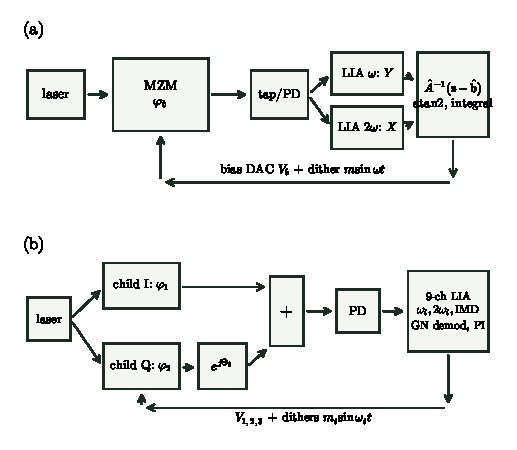
\includegraphics[width=\columnwidth]{figs/fig_arch.pdf}
\caption{Control architectures. (a)~Single MZM: two lock-in channels
feed the affine inverse and $\atan$ demodulator. (b)~DPMZM: nine
lock-in channels (harmonics and intermodulation tones) feed the
Gauss--Newton demodulator of Section~\ref{sec:gn}.}
\label{fig:arch}
\end{figure}

\begin{figure}[!t]
\centering
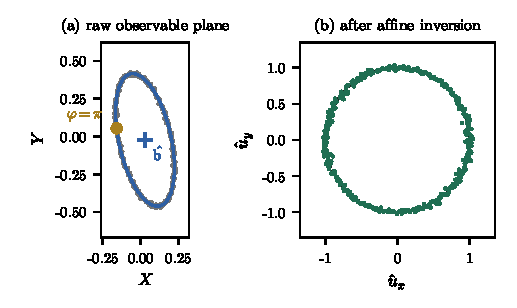
\includegraphics[width=\columnwidth]{figs/fig_ellipse.pdf}
\caption{Calibration at $m{=}1.2$, $\sigma{=}0.005$, $N{=}360$ with
gain imbalance, $10^\circ$ non-orthogonality, cross-coupling
$\varepsilon{=}0.10$, and offsets. (a)~Raw observable plane with fitted
ellipse, center $\hat\bv$, and $\varphi{=}\pi$ fiducial. (b)~Pulled-back
samples $\hat\uv=B(\zv-\hat\bv)$ on the unit circle.}
\label{fig:ellipse}
\end{figure}

\subsection{Closed Loop with Uniform Gain}
With $e=\operatorname{wrap}_{(-\pi,\pi]}(\hat\varphi_b-\varphi^\ast)$,
the error is \emph{identically} linear in the state and independent of
the target when the model holds; with the constant actuator slope
$\partial\varphi_b/\partial V_b=\pi/V_\pi$, one PI(D) tuning serves all
targets with identical bandwidth and margins. Table~\ref{tab:schemes}
collects the unified comparison; the static errors of all conventional
schemes are the closed forms
\eqref{eq:staticQ}--\eqref{eq:staticAM}.

\begin{table}[!t]
\caption{Unified Comparison of Locking Schemes (Single MZM)}
\label{tab:schemes}
\centering
\scriptsize
\setlength{\tabcolsep}{2pt}
\begin{tabular}{lllll}
\toprule
Scheme & Lockable set & Gain & Static error & Ambiguity\\
\midrule
H2 zero (quad) & $\{\pi/2,3\pi/2\}$ & $\eta\kappa_2$ &
$(A_{12}{+}b_X)/A_{11}$ & half-period\\
H1 zero (null/peak) & $\{0,\pi\}$ & $\eta\kappa_1$ &
$(b_Y{-}A_{21})/A_{22}$ & half-period\\
Amplitude match & off dead zones & $\eta\kappa_1|\cos\varphi^\ast|$ &
Eq.~\eqref{eq:staticAM} & $\varphi\!\leftrightarrow\!\pi{-}\varphi$\\
Harmonic ratio & $Y$ not small & target-dep. & $\bv$-dominated &
two-quadrant\\
\textbf{Affine (this work)} & $[0,2\pi)$ & uniform & $0$ (in model) &
none\\
\bottomrule
\end{tabular}
\end{table}

\section{Noise and Dither-Depth Design}
\label{sec:noise}
Perturbing \eqref{eq:affine} along the tangent
$\tv(\varphi)=(-\sin\varphi,\cos\varphi)^{\T}$,
\begin{equation}
\sigma^2_{\hat\varphi}(\varphi)
=\tv^{\T}A^{-1}\Sigma_nA^{-\T}\tv
\xrightarrow{\Sigma_n=\sigma^2I}\sigma^2\,\tv^{\T}M\tv
\le\frac{\sigma^2}{\sigma^2_{\min}(A)},
\label{eq:var}
\end{equation}
with condition number
$\kappa(A)=\sqrt{\lambda_{\max}(M)/\lambda_{\min}(M)}$. In the ideal
chain $\kappa(A)=J_1(m)/J_2(m)\to 4/m$ for small $m$
(Fig.~\ref{fig:bessel}): small dithers make the ellipse flat and
amplify H2-channel noise as $1/J_2\approx 8/m^2$, while the dither
itself costs modulation impairment $\propto m^2$; the trade-off, fully
captured by the single scalar $\kappa(A)$, sets the design of $m$. The
plug-in estimator \eqref{eq:demod} is consistent but not efficient; the
Fisher information is $\sigma^{-2}\|A\tv\|^2$ and the Mahalanobis
projection onto the ellipse attains the Cram\'er--Rao bound, the
difference being second order for moderate $\kappa(A)$. The framework
does not lower the noise floor \emph{at} the special points---there it
reproduces $\sigma_Y/(\eta\kappa_1)$ and
$\sigma_X/(\eta\kappa_2)$---it renders \emph{all other points}
reachable with bounded noise.

\begin{figure}[!t]
\centering
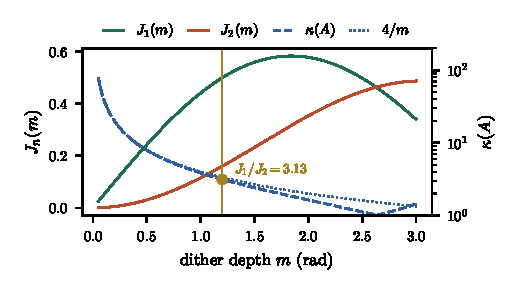
\includegraphics[width=\columnwidth]{figs/fig_bessel.pdf}
\caption{Design curves: $J_1(m)$, $J_2(m)$ (left axis) and the
condition number $\kappa(A)=J_1/J_2$ with its small-$m$ asymptote $4/m$
(right axis, log). Vertical line: $m{=}1.2$ used in the simulations,
giving $\kappa(A)=2.59$.}
\label{fig:bessel}
\end{figure}

\begin{figure}[!t]
\centering
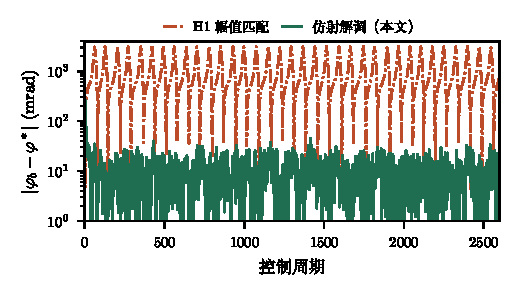
\includegraphics[width=\columnwidth]{figs/fig_mzmloop.pdf}
\caption{Single-MZM closed loop at the arbitrary target
$\varphi^\ast{=}1.9$~rad under identical drift, $\sigma{=}0.005$.
Affine demodulation holds $12.7$~mrad rms; H1 amplitude matching locks
to the wrong branch (static error ${\sim}1.3$~rad).}
\label{fig:mzmloop}
\end{figure}

\section{Extension to the DPMZM: Geometry on $\mathbb{T}^3$}
\label{sec:dpmzm}

\subsection{Field Model and Half-Angle Structure}
The DPMZM nests two child MZMs in a parent interferometer with bias
phases $\phiv=(\varphi_1,\varphi_2,\varphi_3)$. Without RF data,
\begin{align}
E_{\mathrm{out}}&=\frac{E_{\mathrm{in}}}{2}\Bigl[\cos\frac{\Theta_1}{2}
+e^{j\Theta_3}\cos\frac{\Theta_2}{2}\Bigr],\quad \Theta_i=\varphi_i+\xi_i(t),
\nonumber\\
P_{\mathrm{out}}&=\frac{P_0}{8}\bigl[2{+}\cos\Theta_1{+}\cos\Theta_2\bigr]
+\frac{P_0}{2}\cos\frac{\Theta_1}{2}\cos\frac{\Theta_2}{2}\cos\Theta_3.
\label{eq:dpmzm}
\end{align}
The bracket reproduces two single-MZM self terms; the interference
cross term carries \emph{half-angle} factors---the entire structural
difference from the single MZM. Three consequences are immediate:

\emph{(i) $4\pi$ period.} $\cos(\varphi_1/2)$ has period $4\pi$:
$\varphi_1\!\to\!\varphi_1{+}2\pi$ flips the child-I field and the sign
of the cross term, and is intensity-distinguishable. Calibration sweeps
of the child axes must span $4\pi$ (voltage $4V_\pi$), twice the
single-MZM habit.

\emph{(ii) Klein equivalence.} A child field flip combined with a
parent $\pi$ shift changes only the global field sign:
$T_1{:}(\varphi_1{+}2\pi,\varphi_2,\varphi_3{+}\pi)$ and
$T_2{:}(\varphi_1,\varphi_2{+}2\pi,\varphi_3{+}\pi)$ generate
$V_4=\{\mathrm{id},T_1,T_2,T_1T_2\}$; the configuration space is the
quotient $\widetilde{\mathbb{T}}^3/V_4$ (Fig.~\ref{fig:torus}). For
QPSK this equivalence is harmless (constellation relabeling and global
phase).

\emph{(iii)} The standard QPSK bias is
$(\pi,\pi,\pm\pi/2)$ (children at null, parent at quadrature, carrier
suppressed); arbitrary-point operation (microwave-photonic vector
modulation, SSB weighting) parks all three axes at generic values.

\begin{figure}[!t]
\centering
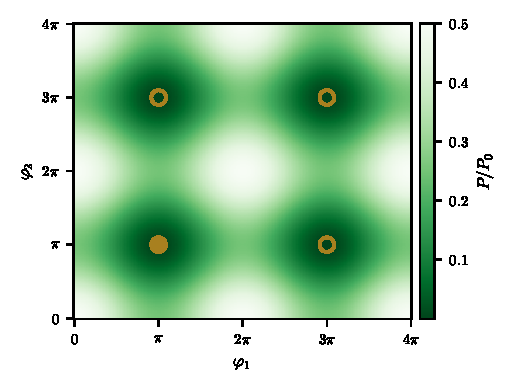
\includegraphics[width=\columnwidth]{figs/fig_torus.pdf}
\caption{DPMZM intensity $P(\varphi_1,\varphi_2;\varphi_3{=}\pi/2)$
over the full $[0,4\pi)^2$ patch. The standard QPSK point (filled) and
its three Klein images (open) are intensity-identical---the $V_4$
quotient made visible.}
\label{fig:torus}
\end{figure}

\subsection{Three-Tone Harvest and the Feature Map}
With dithers $\xi_i=m_i\sin\omega_it$, the self terms expand with
coefficients $J_n(m_i)$ as before, but the cross term expands with
\emph{half-depth} coefficients $j_n^{(i)}\triangleq J_n(m_i/2)$ and
generates intermodulation (IMD) lines
$\omega_1{\pm}\omega_2,\ \omega_3{\pm}\omega_1,\ \omega_3{\pm}\omega_2$,
which are legitimate information-bearing channels rather than
parasitics. Table~\ref{tab:dpchan} lists the leading coefficients of
the nine channels used here ($\rho P_0{=}1$, unit gains;
$c_i{=}\cos\frac{\varphi_i}{2}$, $s_i{=}\sin\frac{\varphi_i}{2}$,
$C_3{=}\cos\varphi_3$, $S_3{=}\sin\varphi_3$). Two observations: the
cross coupling is \emph{not} perturbative
($j_1^{(1)}j_0^{(2)}J_0(m_3)\approx m_1/4$ exceeds the self slope
$J_1(m_1)/4\approx m_1/8$), and the frequency plan must keep the set
$\{\omega_i,2\omega_i,\omega_1{\pm}\omega_2,\omega_3{\pm}\omega_{1,2}\}$
collision-free (here $\omega_{1,2,3}=1,1.37,1.93$).

\begin{table}[!t]
\caption{Leading Coefficients of the Nine DPMZM Channels}
\label{tab:dpchan}
\centering
\scriptsize
\setlength{\tabcolsep}{2pt}
\begin{tabular}{llll}
\toprule
Ch. & Freq. & Leading coefficient $\times$ monomial & Role\\
\midrule
$Y_1$ & $\omega_1$ & $-\frac14J_1^{(1)}\sin\varphi_1-j_1^{(1)}j_0^{(2)}J_0(m_3)\,s_1c_2C_3$ & child-I lock\\
$X_1$ & $2\omega_1$ & $+\frac14J_2^{(1)}\cos\varphi_1+j_2^{(1)}j_0^{(2)}J_0(m_3)\,c_1c_2C_3$ & discriminator\\
$Y_2$ & $\omega_2$ & $-\frac14J_1^{(2)}\sin\varphi_2-j_0^{(1)}j_1^{(2)}J_0(m_3)\,c_1s_2C_3$ & child-Q lock\\
$X_2$ & $2\omega_2$ & $+\frac14J_2^{(2)}\cos\varphi_2+j_0^{(1)}j_2^{(2)}J_0(m_3)\,c_1c_2C_3$ & discriminator\\
$Y_3$ & $\omega_3$ & $-j_0^{(1)}j_0^{(2)}J_1(m_3)\,c_1c_2S_3$ & parent (note $c_1c_2$)\\
$X_3$ & $2\omega_3$ & $+j_0^{(1)}j_0^{(2)}J_2(m_3)\,c_1c_2C_3$ & parent discrim.\\
$Z_-$ & $\omega_1{-}\omega_2$ & $+j_1^{(1)}j_1^{(2)}J_0(m_3)\,s_1s_2C_3$ & Kawakami-type \cite{kawakami2012}\\
$Z_{13}$ & $\omega_3{-}\omega_1$ & $+j_1^{(1)}j_0^{(2)}J_1(m_3)\,s_1c_2S_3$ & this work\\
$Z_{23}$ & $\omega_3{-}\omega_2$ & $+j_0^{(1)}j_1^{(2)}J_1(m_3)\,c_1s_2S_3$ & this work\\
\bottomrule
\end{tabular}
\end{table}

Applying Lemma~\ref{lem:fact} to each phase (the half-angle version
holds verbatim) and expanding the cross term trilinearly, the
$\phiv$-dependence of the photocurrent can only consist of the twelve
trigonometric monomials
\begin{align}
\Phi(\phiv)&=\bigl(\underbrace{\cos\varphi_1,\sin\varphi_1,
\cos\varphi_2,\sin\varphi_2}_{\text{self (full angle)}},\;
\underbrace{\vv_1{\otimes}\vv_2{\otimes}\vv_3}_{\text{cross, 8-dim}}
\bigr),\nonumber\\
\vv_1&=(c_1,s_1),\quad \vv_2=(c_2,s_2),\quad \vv_3=(C_3,S_3).
\label{eq:feature}
\end{align}

\begin{theorem}[DPMZM exact affinity]
\label{th:dpmzm}
For arbitrary periodic dither waveforms $\{\xi_i\}$, any linear receive
chain, and any set of $K$ linear demodulation functionals,
\begin{equation}
\zv=A\,\Phi(\phiv)+\bv+\nv,\qquad A\in\mathbb{R}^{K\times 12},
\label{eq:dpaffine}
\end{equation}
holds exactly. In the ideal chain $A=A_0$ is given by
Table~\ref{tab:dpchan} and is highly sparse (one to two nonzeros per
row, Fig.~\ref{fig:ahat}).
\end{theorem}

A methodological shift accompanies the theorem: in one dimension we
enumerated impairment mechanisms; in three dimensions black-box affine
identification absorbs \emph{all} linear mismatch, and mechanism
enumeration is replaced by the structure theorem. The gauge group also
generalizes verbatim: phase shifts $\varphi_i\to\varphi_i+\alpha_i$ act
\emph{linearly} on the feature space (half-angle pairs rotate by
$\alpha_i/2$, full-angle pairs by $\alpha_i$, the tensor block by the
tensor rotation), so $(A,\bv)$ is identifiable up to three phase
origins---fixed per axis by dc regression exactly as in
Section~\ref{sec:calib}---plus reflections (sweep orientation) and the
discrete $V_4$ (fundamental-domain convention).
Table~\ref{tab:struct} summarizes the correspondence.

\begin{table}[!t]
\caption{Structural Correspondence: Single MZM vs.\ DPMZM}
\label{tab:struct}
\centering
\footnotesize
\setlength{\tabcolsep}{4pt}
\begin{tabular}{lll}
\toprule
Element & Single MZM & DPMZM\\
\midrule
State manifold & $\mathbb{S}^1$ & $\mathbb{T}^3$ (config.\ $\widetilde{\mathbb{T}}^3/V_4$)\\
Feature map & $\uv\in\mathbb{R}^2$ (identity) & $\Phi\in\mathbb{R}^{12}$ (half angles)\\
Axis period & $2\pi$ & children $4\pi$, parent $2\pi$\\
Channels & 2 ($\omega,2\omega$) & $\ge 7$, IMD mandatory\\
Surface fitting & ellipse (quadric) & regression on quasi-periodic sweep\\
Gauge group & $O(2)$ & $\mathbb{T}^3\rtimes(\text{refl.}\times V_4)$\\
Demodulation & $\atan$ (closed form) & warm-started Gauss--Newton\\
Blindness cure & H1/H2 jointly & IMD channels\\
\bottomrule
\end{tabular}
\end{table}

\section{Observability and the Necessity of IMD Channels}
\label{sec:obs}
Local demodulability is governed by the observation Jacobian
$\Jc(\phiv)=A\,D\Phi(\phiv)\in\mathbb{R}^{K\times3}$ through the rank
condition $\sigma_{\min}(\Jc)>0$---the direct generalization of the
immersion argument of Proposition~\ref{prop:rolle}. Unlike the circle,
the \emph{observed} embedding of $\mathbb{T}^3$ can degenerate, and it
does so at the worst possible place.

\begin{proposition}[Standard-point blindness and its locus]
\label{prop:blind}
Consider the six harmonic channels $Y_{1,2,3},X_{1,2,3}$ of
Table~\ref{tab:dpchan} with the ideal $A_0$. The set on which
$\partial\zv/\partial\varphi_3=\mathbf{0}$ (parent axis unobservable)
is exactly $\{c_1=c_2=0\}$, i.e., \emph{the Klein orbit of the standard
QPSK operating point}, for every $\varphi_3$. Adding the IMD channel
$Z_-$ (monomial $s_1s_2C_3$, whose $\varphi_3$-derivative
$-s_1s_2S_3=\mp1$ at the standard point) restores full rank there.
\end{proposition}
\begin{proof}[Proof sketch]
The $\varphi_3$-derivatives reaching the six channels are
$-s_1c_2S_3$ ($Y_1$), $-c_1s_2S_3$ ($Y_2$), $-c_1c_2S_3$
($X_1,X_2,X_3$), and $+c_1c_2C_3$ ($Y_3$). Their simultaneous vanishing
for all $\varphi_3$ requires $s_1c_2=c_1s_2=c_1c_2=0$, whose only
solutions are $c_1=c_2=0$ (the alternative $s_1=s_2=0$ contradicts
$c_1c_2=0$). Numerically,
$\sigma_{\min}=1.3\times10^{-9}$ (machine zero) for the six channels at
$(\pi,\pi,\pi/2)$ versus $5.5\times10^{-2}$ with $Z_-$ included.
\end{proof}

The conventional channel set is thus not ``occasionally'' degenerate:
it is blind \emph{precisely} at the point where every QPSK transmitter
operates. The IMD detection of the parent bias used in the literature
\cite{kawakami2012} is therefore a rank-condition necessity. A residual
singularity remains for honesty's sake: on
$\{c_1{=}c_2{=}0,\ S_3{=}0\}$ (e.g., $(\pi,\pi,0)$, output dark) all
$\varphi_3$-derivatives fall on the single unobserved monomial
$s_1s_2S_3$ and $\sigma_{\min}=1.1\times10^{-17}$ even with nine
channels; third-order IMD $\omega_1{+}\omega_2{\pm}\omega_3$ or path
detours resolve it. Fig.~\ref{fig:obs} maps
$\log_{10}\sigma_{\min}(\Jc)$ over $[0,4\pi)^2$: dark spots at the
Klein orbit for six channels, full repair with nine channels at
$\varphi_3=\pi/2$, and the predicted residual spots at $\varphi_3=0$.

\begin{figure*}[!t]
\centering
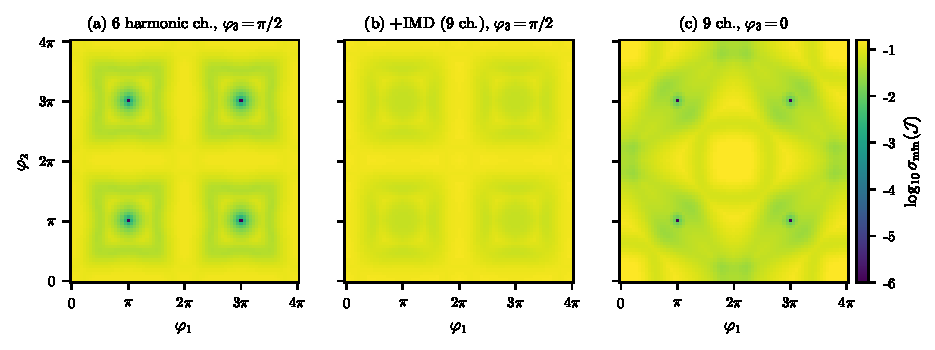
\includegraphics[width=0.95\textwidth]{figs/fig_obs.pdf}
\caption{Observability maps $\log_{10}\sigma_{\min}(\Jc)$ over
$(\varphi_1,\varphi_2)\in[0,4\pi)^2$. (a)~Six harmonic channels,
$\varphi_3{=}\pi/2$: blind spots exactly on the Klein orbit of the
standard QPSK point. (b)~Adding the three IMD channels repairs them.
(c)~Nine channels at $\varphi_3{=}0$: the residual singularity of
Proposition~\ref{prop:blind} appears on the same orbit.}
\label{fig:obs}
\end{figure*}

\section{Calibration and Gauss--Newton Demodulation on $\mathbb{T}^3$}
\label{sec:gn}
The single-MZM calibration exploited the accident that the model
surface is a quadric. $\Phi(\mathbb{T}^3)$ is not, and geometric
fitting loses its closed form---but the theorem compensates:
observations are \emph{linear in the features}, so with gauge-fixed
sweep phases the identification is ordinary least squares,
\begin{equation}
[\hat A\,|\,\hat\bv]
=\Bigl(\sum_k\zv_k\tilde\Phi_k^{\T}\Bigr)
\Bigl(\sum_k\tilde\Phi_k\tilde\Phi_k^{\T}\Bigr)^{-1},\quad
\tilde\Phi=\begin{pmatrix}\Phi\\1\end{pmatrix},
\label{eq:regress}
\end{equation}
one $13{\times}13$ Gram factorization serving all $K$ channels. A 3-D
grid sweep is unnecessary: a single \emph{quasi-periodic} trajectory
$\varphi_i(k)=k\Delta_i$ with irrational increment ratios (here
$\Delta=(0.0424,0.0532,0.0679)$) fills $\mathbb{T}^3$ ergodically;
$N=3000$ samples give a well-conditioned Gram matrix. Per-axis scales
$V_{\pi,i}$ come from fundamental-period estimation of the sweep data
(child axes: period $4\pi$), and the absolute origins---the
$\mathbb{T}^3$ gauge---from per-axis dc regression as before.

Demodulation generalizes $\atan$, which exists because the circle
embedding has a global closed-form inverse; $\Phi(\mathbb{T}^3)$ has
none, but control is a \emph{tracking} problem: the previous estimate
warm-starts a damped Gauss--Newton step \cite{nocedal2006}
\begin{equation}
\hat\phiv\leftarrow\hat\phiv+(\Jc^{\T}\Jc+\lambda I)^{-1}
\Jc^{\T}\bigl[\zv-\hat A\Phi(\hat\phiv)-\hat\bv\bigr],
\label{eq:gn}
\end{equation}
two iterations of which reach the measurement-noise floor; the
convergence basin is governed by $\sigma_{\min}(\Jc)$ and the embedding
curvature, so the maps of Fig.~\ref{fig:obs} double as convergence-basin
charts. Owing to the sparsity of $\hat A$ the cost is a few hundred
multiply--accumulates plus a $3{\times}3$ solve per control
cycle---negligible on a Cortex-M class controller next to the lock-in
processing itself. The error $\mathbf{e}=\hat\phiv-\phiv^\ast$ is again
exactly linear, axis-decoupled, and target-independent.

As the conventional baseline we adopt the literature-style three
independent loops: error quantities $(Y_1,Y_2,Z_-)$, reference values
from the ideal model $A_0\Phi(\phiv^\ast)$, and the \emph{diagonal}
entries of the ideal Jacobian as slopes---i.e., the designer
acknowledges the ideal coupling but forgoes matrix inversion, and is
ignorant of $A\neq A_0$, $\bv\neq0$. Near the standard point this
baseline is free of coupling (the cross terms vanish there locally,
giving the geometric explanation of why the textbook design works at
all), but it inherits the static errors of Section~\ref{sec:conventional}
amplified by the second-order-small parent slope
$j_1^{(1)}j_1^{(2)}J_0(m_3)$; at arbitrary targets, cross-axis coupling
and dead zones are added on top.

\begin{figure}[!t]
\centering
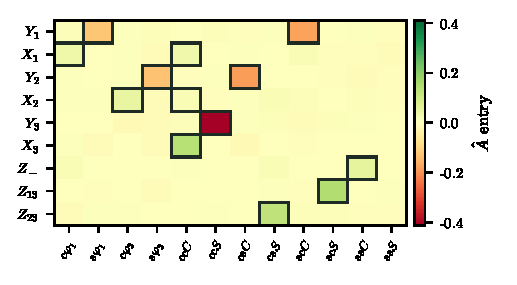
\includegraphics[width=\columnwidth]{figs/fig_ahat.pdf}
\caption{Black-box identification of the DPMZM: the regressed $\hat A$
(color) against the sparsity fingerprint of the ideal $A_0$ (boxes).
Off-fingerprint entries are the injected unstructured perturbation
$\delta_A{=}0.12$, faithfully captured.}
\label{fig:ahat}
\end{figure}

\section{Numerical Validation}
\label{sec:numerics}
All simulations generate data from a perturbed truth
$A_{\mathrm{true}}=A_0+\delta_A\,\Delta A$,
$\bv_{\mathrm{true}}=\delta_b\,\Delta\bv$ with fixed pseudo-random
$\Delta A,\Delta\bv$ ($\delta_A{=}0.12$ relative Frobenius scale,
$\delta_b$ giving offsets of ${\sim}10^{-2}$), per-channel Gaussian
noise, and a common drift sequence (random walk plus slow sinusoids)
applied to all controllers under comparison. Single-MZM parameters:
$m{=}1.2$, $g_X{=}1.18$, $g_Y{=}0.88$, $\delta{=}10^\circ$,
$\varepsilon{=}0.10$, $\bv=(0.030,-0.022)$, $\sigma{=}0.005$,
$N{=}360$; DPMZM: $m_i{=}1.2$, $\sigma{=}0.002$, $N{=}3000$.
Table~\ref{tab:results} summarizes.

\begin{table}[!t]
\caption{Numerical Validation Summary}
\label{tab:results}
\centering
\scriptsize
\setlength{\tabcolsep}{2.5pt}
\begin{tabular}{ll}
\toprule
Quantity & Result\\
\midrule
\multicolumn{2}{l}{\emph{Single MZM}}\\
Noiseless demod.\ error (full period) & $0.0000$ mrad (machine prec.)\\
Noiseless $\hat A$ vs.\ true $A$ & $0.00\%$ Frobenius\\
Noisy cal.\ demod.\ bias ($\sigma{=}0.005$) & median $2.35$, P95 $6.25$ mrad\\
Gauge: dc regression vs.\ argmin & ${\sim}2.4$ vs.\ ${\sim}30$ mrad\\
Closed loop @ $\varphi^\ast{=}1.9$ & affine $12.7$ / H1-match $1315$ mrad rms\\
$\kappa(A)$ at $m{=}1.2$ & $2.59$\\
\midrule
\multicolumn{2}{l}{\emph{DPMZM}}\\
$D\Phi$ vs.\ finite differences & $8\times10^{-10}$ max\\
Klein invariance $\|\Phi\circ T_1-\Phi\|$ & $2\times10^{-15}$\\
Noiseless identification / GN recovery & $2.4\times10^{-13}\%$ / $6\times10^{-12}$ mrad\\
Noisy ident.\ ($\sigma{=}0.002$) / demod.\ bias & $0.17\%$ / median $1.9$, P95 $3.8$ mrad\\
$\sigma_{\min}$: 6ch / 9ch @ std.\ pt. & $1.3\times10^{-9}$ / $5.5\times10^{-2}$\\
$\sigma_{\min}$: 9ch @ $(\pi,\pi,0)$ & $1.1\times10^{-17}$\\
Closed loop, arbitrary target & GN $17.2$ / 3-loop $358$ mrad rms\\
Closed loop, standard target & GN $18.5$ / 3-loop $397$ mrad rms\\
3-loop static error, 30 realizations & std.: med.\ $274$ [184,373] mrad\\
 & arb.: med.\ $749$ mrad, Q3 diverges\\
\bottomrule
\end{tabular}
\end{table}

Three results deserve emphasis. First, the noiseless closures
($10^{-13}\%$ identification, $10^{-12}$~mrad demodulation from
$0.3$~rad warm-start offsets) confirm that
Theorems~\ref{th:affine}--\ref{th:dpmzm} are exact rather than
approximate statements. Second, the closed-loop comparison
(Figs.~\ref{fig:mzmloop} and~\ref{fig:dploop}) exhibits the layered
failure of conventional control predicted by the theory: at the
arbitrary single-MZM target the H1 scheme locks the wrong branch; for
the DPMZM the three-loop baseline converges in both cases but carries
static errors of several hundred mrad dominated by the unidentified
$(\Delta A,\bv)$ acting through the small parent slope---a Monte-Carlo
over 30 mismatch realizations gives a median static error of 274~mrad
at the standard point and 749~mrad at the arbitrary target, with the
upper quartile of the latter diverging (loss of lock)---while the
Gauss--Newton affine controller holds $17$--$19$~mrad rms in all cases,
limited only by measurement noise. Third, the observability maps
(Fig.~\ref{fig:obs}) visualize Proposition~\ref{prop:blind} exactly:
the six-channel blind spots sit on the Klein orbit of the standard
point, are repaired by the IMD channels, and the predicted residual
singularity reappears on the $S_3{=}0$ slice.

\begin{figure*}[!t]
\centering
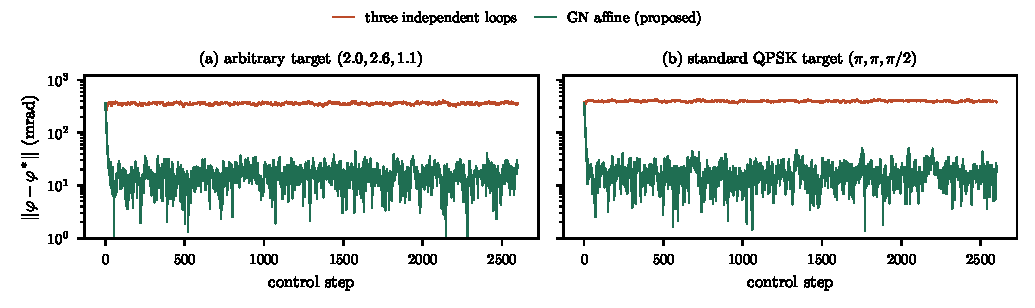
\includegraphics[width=0.95\textwidth]{figs/fig_dploop.pdf}
\caption{DPMZM closed-loop tracking under identical drift,
$\sigma{=}0.002$, $\delta_A{=}0.12$. (a)~Arbitrary target: the
three-loop baseline carries a ${\sim}0.36$~rad static error; (b)~even
at the standard QPSK target the baseline inherits a comparable static
error through the second-order-small parent slope, while the
Gauss--Newton affine controller holds ${\sim}18$~mrad rms in both
cases.}
\label{fig:dploop}
\end{figure*}

\subsection{Noise Floor and Dither Design on $\mathbb{T}^3$}
The estimate covariance is Cram\'er--Rao-type,
$\Sigma_{\hat\phiv}=(\Jc^{\T}\Sigma_n^{-1}\Jc)^{-1}$, of which
\eqref{eq:var} is the $K{=}2$ degeneration. The conditioning is now
dominated by the second-order-small IMD coefficient: near the
children-null region the parent-phase variance is
\begin{equation}
\sigma^2_{\hat\varphi_3}\approx
\frac{\sigma^2}{\bigl[j_1^{(1)}j_1^{(2)}J_0(m_3)\bigr]^2}
\approx\Bigl(\frac{16}{m_1m_2}\Bigr)^{2}\sigma^2,
\label{eq:parentnoise}
\end{equation}
an order of magnitude above the child floor $(8/m)^2\sigma^2$ and
quadratic rather than linear in $1/m$. The dither depth is therefore
set by the parent-axis IMD signal-to-noise ratio, not by the children,
and the optimum sits markedly above single-MZM habits.

\section{Discussion}
\label{sec:discussion}
\emph{Persistent excitation.} In closed-loop steady state $\phiv$
parks at one point and $(A,\bv)$ loses observability---common to all
identification-based schemes \cite{ljung1999}. Practical remedies:
residual monitoring
$\|\zv-\hat A\Phi(\hat\phiv)-\hat\bv\|$ as a mismatch alarm triggering
recalibration; periodic micro-arcs (drift transients themselves are
natural excitation); subspace-restricted recursive least squares. On
$\mathbb{T}^3$ the recalibration arcs should preferentially excite the
IMD-related subspace ($s_1s_2$ directions), whose coefficients are the
weakest and whose drift is identified the slowest.

\emph{DP-QPSK.} A dual-polarization transmitter is two DPMZMs. With
independent monitor photodiodes per polarization the model is exactly
block-diagonal---two parallel instances of this framework with no
coupling, formalizing the X/Y decoupling as the key dimensionality
reduction of the six-bias problem and quantifying the value of
per-polarization monitoring. A shared photodiode adds
inter-polarization beat terms: the theorem form survives with an
enlarged feature space (a subset of the tensor product of the two
$\Phi$'s) at a dimensional cost.

\emph{Hardware.} For an existing dual-harmonic (H1/H2) STM32-class
lock-in firmware, the single-MZM scheme is a pure software upgrade: one
boot-time calibration sweep, a $2{\times}2$ multiply--add, and one
$\atan$ lookup per cycle; the six calibration scalars
$(\hat A,\hat\bv)$ fit in a configuration page. The DPMZM scheme adds
the IMD lock-ins and the sparse $9{\times}12$ Gauss--Newton step, in
total under $10^3$ MACs per cycle.

\emph{Limitations.} The framework is exact only as far as the two
linearity assumptions of Section~\ref{sec:affine}; photodiode/TIA
nonlinearity and bias-dependent absorption produce non-affine residuals
that bound the absolute accuracy together with the
$O(\varepsilon)$ gauge shift of the dc fiducial. The Klein quotient and
the $4\pi$ period must be respected by the supervisory logic
(fundamental-domain bookkeeping); and cold-start demodulation on
$\mathbb{T}^3$ requires a coarse seed search (the $V_4$ images are
acceptable seeds since they are physically equivalent).

\section{Conclusion}
A single identity---the factorization of the bias phase out of the
dithered transfer function---forces the harmonically demodulated
observables of an MZM to be an exact affine image of the circle, and
those of a DPMZM to be an exact affine image of a 12-dimensional
trigonometric embedding of the 3-torus. Everything else follows:
conventional special-point locking and its static errors are degenerate
readouts of the affine model; arbitrary-point control reduces to
identification plus inversion with target-independent loop gain; the
IMD detection of the DPMZM parent bias is a rank-condition necessity
whose precise singular locus is the Klein orbit of the standard QPSK
point; and the calibration and demodulation algorithms scale from
ellipse-fit-plus-$\atan$ to quasi-periodic-regression-plus-Gauss--Newton
at microcontroller cost. The structural theorems organize a family of
scattered engineering techniques as projections of one geometric fact,
and the numerical validation confirms them at machine precision.

\appendices
\section{Leading-Order Entries Under Dither Distortion}
\label{app:eps}
Let $\xi=m\sin\omega t+\varepsilon m\sin(2\omega t+\psi)$ and expand
$\cos\xi\approx\cos(m\sin\omega t)-\delta\xi\sin(m\sin\omega t)$,
$\sin\xi\approx\sin(m\sin\omega t)+\delta\xi\cos(m\sin\omega t)$ with
$\delta\xi=\varepsilon m\sin(2\omega t+\psi)$. Using
$\cos(m\sin\omega t)=J_0+2\sum_{k\ge1}J_{2k}\cos2k\omega t$ and
$\sin(m\sin\omega t)=2\sum_{k\ge0}J_{2k+1}\sin(2k{+}1)\omega t$, the
products contribute at $\omega$ via
$\sin(2\omega t{+}\psi)\sin\omega t$ and
$\sin(2\omega t{+}\psi)\sin3\omega t$, and at $2\omega$ via
$\sin(2\omega t{+}\psi)\cdot J_0$ and
$\sin(2\omega t{+}\psi)\cos4\omega t$. With the projection identity
$\overline{2\sin(n\omega t{+}\alpha)\cos(n\omega t{+}\beta)}
=\sin(\alpha-\beta)$ one obtains
\begin{align}
\Lc_1[\cos\xi]&=-\varepsilon m\bigl[J_1\sin(\theta_1{-}\psi)
+J_3\sin(\theta_1{+}\psi)\bigr],\nonumber\\
\Lc_1[\sin\xi]&=2J_1\cos\theta_1+O(\varepsilon^2),\nonumber\\
\Lc_2[\cos\xi]&=2J_2\cos\theta_2+O(\varepsilon^2),\nonumber\\
\Lc_2[\sin\xi]&=\varepsilon m\bigl[J_0\sin(\psi{-}\theta_2)
+J_4\sin(\psi{+}\theta_2)\bigr],
\end{align}
which, inserted in \eqref{eq:entries}, give \eqref{eq:Aeps}: at
$O(\varepsilon)$ the distortion leaves the diagonal untouched and
populates only the off-diagonal. The same expansion applied to the dc
component yields the fiducial phase shift
$\delta\varphi_c\approx\varepsilon mJ_2(m)\sin\psi/J_0(m)$ quoted in
Section~\ref{sec:calib}.

\begin{thebibliography}{10}

\bibitem{salvestrini2011}
J.~P. Salvestrini, L.~Guilbert, M.~Fontana, M.~Abarkan, and S.~Gille,
``Analysis and control of the {DC} drift in {LiNbO$_3$}-based
{Mach--Zehnder} modulators,'' \emph{J. Lightw. Technol.}, vol.~29,
no.~10, pp. 1522--1534, May 2011.

\bibitem{chen2011}
A.~Chen and E.~J. Murphy, Eds., \emph{Broadband Optical Modulators:
Science, Technology, and Applications}.\hskip 1em plus 0.5em minus
0.4em\relax Boca Raton, FL, USA: CRC Press, 2011.

\bibitem{cho2006}
P.~S. Cho, J.~B. Khurgin, and I.~Shpantzer, ``Closed-loop bias control
of optical quadrature modulator,'' \emph{IEEE Photon. Technol. Lett.},
vol.~18, no.~21, pp. 2209--2211, Nov. 2006.

\bibitem{sotoodeh2011}
M.~Sotoodeh, Y.~Beaulieu, J.~Harley, and D.~L. McGhan, ``Modulator bias
and optical power control of optical complex {E}-field modulators,''
\emph{J. Lightw. Technol.}, vol.~29, no.~15, pp. 2235--2248, Aug. 2011.

\bibitem{kawakami2012}
H.~Kawakami, E.~Yoshida, and Y.~Miyamoto, ``Auto bias control technique
based on asymmetric bias dithering for optical {QPSK} modulation,''
\emph{J. Lightw. Technol.}, vol.~30, no.~7, pp. 962--968, Apr. 2012.

\bibitem{heydemann1981}
P.~L.~M. Heydemann, ``Determination and correction of quadrature fringe
measurement errors in interferometers,'' \emph{Appl. Opt.}, vol.~20,
no.~19, pp. 3382--3384, 1981.

\bibitem{fitzgibbon1999}
A.~Fitzgibbon, M.~Pilu, and R.~B. Fisher, ``Direct least square fitting
of ellipses,'' \emph{IEEE Trans. Pattern Anal. Mach. Intell.}, vol.~21,
no.~5, pp. 476--480, May 1999.

\bibitem{yao2009}
J.~Yao, ``Microwave photonics,'' \emph{J. Lightw. Technol.}, vol.~27,
no.~3, pp. 314--335, Feb. 2009.

\bibitem{nocedal2006}
J.~Nocedal and S.~J. Wright, \emph{Numerical Optimization}, 2nd
ed.\hskip 1em plus 0.5em minus 0.4em\relax New York, NY, USA: Springer,
2006.

\bibitem{ljung1999}
L.~Ljung, \emph{System Identification: Theory for the User}, 2nd
ed.\hskip 1em plus 0.5em minus 0.4em\relax Upper Saddle River, NJ, USA:
Prentice Hall, 1999.

\end{thebibliography}

\end{document}
